\documentclass{beamer}

\author{Yu Cong}
\title[Minimizing sum of pwl convex function]{Minimizing the Sum of Piecewise Linear Convex Functions}
\date{\today}

% \AtBeginSection[]{
%     \frame{\frametitle{Outline}\tableofcontents[currentsection, 
%     subsectionstyle=show/show/shaded]}
% }
    
\usetheme{Simple}
% \useoutertheme{tree}
    
\begin{document}
\begin{frame}[plain]
    % Print the title page as the first slide
    \titlepage
\end{frame}

\begin{frame}[plain]{Plan}
    \mybox[oliver!10]{\scriptsize The order of the slides is basically the order in which I think about this problem.}
    \tableofcontents
\end{frame}

\section{Problems \& Definitions}
\begin{frame}{$\min \sum f_i(a_i\cdot x-b_i)$}
\begin{problem}
    Given $n$ piecewise linear convex functions $f_1,...,f_n:\R \to \R$ of total $m$ breakpoints, and $n$ linear functions $a_i\cdot x-b_i:\R^d\to \R$, find $\min_x \sum_i f_i(a_i\cdot x-b_i)$.
\end{problem}
\begin{figure}
    \centering
    \begin{subfigure}{.5\textwidth}
      \centering
      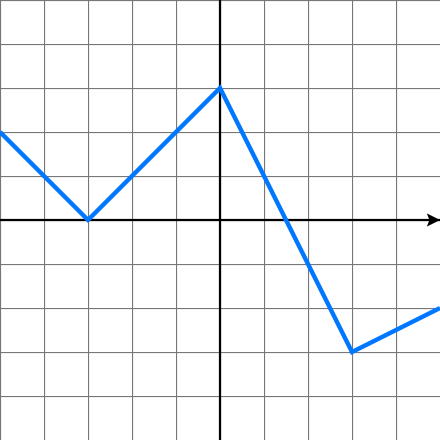
\includegraphics[width=.4\linewidth]{images/Piecewise_linear_function.svg.png}
      \caption{A 1D piecewise linear function with 4 line segments and 3 breakpoints}
      \label{fig:sub1}
    \end{subfigure}%
    \begin{subfigure}{.5\textwidth}
      \centering
      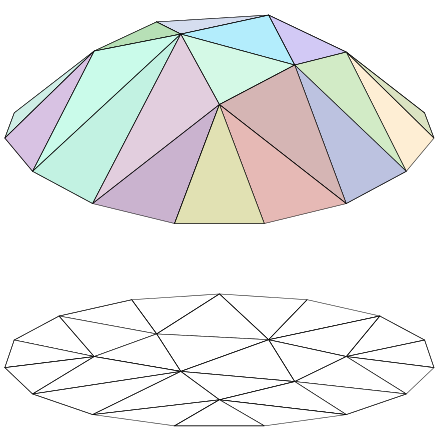
\includegraphics[width=.4\linewidth]{images/Piecewise_linear_function2D.png}
      \caption{A 2D piecewise concave function}
      \label{fig:sub2}
    \end{subfigure}
    % \caption{A figure with two subfigures}
    \label{fig:1}
    \end{figure}
    $f_i(a_i\cdot x-b_i):\R^d\to \R$ is also piecewise linear convex.
\end{frame}

\begin{frame}{General piecewise linear convex function in $\R^d$}
\begin{definition}[piecewise linear convex function in $\R^d$]\label{def:pwlc}
\[
g(x)=\max \{a_1^Tx+b_1,\ldots,a_L^Tx+b_L\}
\]
\end{definition}

Every piecewise linear convex function in $\R^d$ can be expressed in this form.\footnote{S.P. Boyd, L. Vandenberghe, \textbf{Convex optimization}, Cambridge University Press, Cambridge, UK ; New York, 2004.}

However, observe that in our problem the piecewise linear convex function is not that general. It is a composition of a linear mapping and an 1D piecewise linear convex function.

\end{frame}

\begin{frame}{$f\circ l\not \equiv g$}
    \begin{proof}
    \small
    Consider a piecewise linear convex function $g:\R^2\to \R$. $g$ can be viewed as the maximum of a set of planes in $\R^3$.

    Consider a series of points $P=\set{p_1,p_2,...,p_k}$ on the 2D plane. After applying the linear mapping to $P$, we will get a sequence of numbers(points in 1D) $P'=\set{p_1',p_2',...,p_k'}$. We assume that $P'$ is non-decreasing. Note that the value of $g$ on $P'$ is always unimodal since $g$ is convex. However, the value of $f$ on $P$ may not be unimodal. Thus the composition of a linear mapping and a pwl convex function in 1D is not equivalent to pwl convex functions in high dimensions.
    \end{proof}
\end{frame}

\section{Properties}
\begin{frame}[allowframebreaks]{A linear time algorithm}
    \begin{problem}
        Given $n$ piecewise linear convex functions $f_1,...,f_n:\R \to \R$ of total $m$ breakpoints, and $n$ linear functions $a_i\cdot x-b_i:\R^d\to \R$, find $\min_x \sum_i f_i(a_i\cdot x-b_i)$.
    \end{problem}
    This can be solve in $O(2^{2^d} (m+n))$ through Megiddo's Low dimension LP algorithm.\footnote{Nimrod Megiddo. Linear programming in linear time when the dimension is fixed. J. ACM, 31(1):114–127, jan 1984.}

    Let $n_i$ be the number of line segments in $f_i$. Note that $\sum_i n_i=m+n$.

    We can formulate the optimization problem as the following linear program,
    \newpage

    \begin{align*}
        \min &\sum_{i=1}^n f_i\\
        s.t. \quad f_i&\geq \alpha_j(a_i\cdot x -b_i)-\beta_j \quad \forall i\in[n], \forall j\\
    \end{align*}

    where $\alpha_j x - \beta_j$ is the $j$'th line segment on $f_i$.

    There will be $m+n$ constraints in total.
\end{frame}

\section{LP in Low Dimensions}
\begin{frame}[allowframebreaks]{Megiddo's algorithm}
    {\tiny \url{https://people.inf.ethz.ch/gaertner/subdir/texts/own_work/chap50-fin.pdf}}

    The dimension $d$ (in our problem, the dimension of $x$) is small while the number of constraints are huge. We need only $d$ linearly independent tight constraints to identify the optimal solution $x^*$.
    Thus most of the constraints are useless.
    \BlankLine


    \textbf{For one constraint, how can we know where does $x^*$ locate with respect to it?}

    Through inquiries. Let $a\cdot x \leq b$ be the constraint. Define 3 hyperplanes, $a\cdot x = c$ where $c\in \set{b,b-\e,b+\e}$. Now solve three $d-1$ dimension linear programming. The largest of the three objective functions tells us where $x^*$ lies with respect to the
    hyperplane.

    \newpage
    Finding the optimal solution $x^*$ is therefore equivalent to the following problem,
    \begin{problem}[Multidimensional Search Problem]
        Suppose that there exists a point $x^*$ which is not known to us, but there is a oracle that can tell the position of $x^*$ relative to any hyperplane in $\R^d$. Given $n$ hyperplanes, we want to know the position of $x^*$ relative to each of them.
    \end{problem}

    \textbf{What about 1 dimension search?} A fastest way will be using the linear time median algorithm. We can find the median of $n$ numbers and call the oracle to compare the median with $x^*$. Thus with $O(n)$ time median finding and one oracle call, we find the relative position of $n/2$ elements relative to $x^*$.

    \newpage

    If we can do similar things in $\R^d$, i.e., there is a method which makes $A(d)$ oracle calls and determines at least $B(d)$ fraction of relative positions, then we can apply this method $\log_{\frac{1}{1-B(d)}} n$ times to find all relative positions.

    Note that in 1 dimension, $A(1)=1$ and $B(1)=1/2$ (call oracle to compare $x^*$ and the median). In $\R^d$, our oracle is the recursive inquiry.

    A trivial method will be iterating on all hyperplanes and calling the oracle on each one, since there is no \emph{median} of a set of hyperplanes in $\R^d$. The complexity recurrence is 
    \[T(n,d)=n(3T(n-1,d-1)+O(nd))\] 
    Note that in this setting $A(d)=1$ and $B(d)=1/n$.

    \newpage
    Megiddo designed a clever method where $A(d)=2^{d-1}$ and $B(d)=2^{-(2^d-1)}$.

    \begin{lemma}
        \begin{figure}
            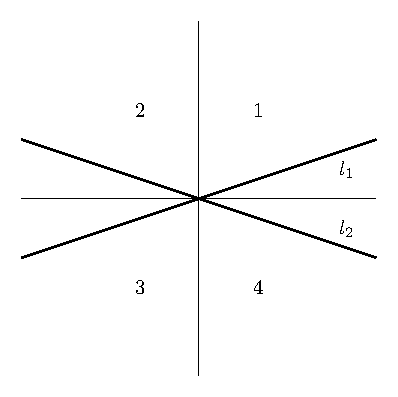
\includegraphics[width=.3\textwidth]{images/1234.pdf}
        \end{figure}
        Given two lines through the origin with slopes of opposite sign, knowing which quadrant $x^*$ lies in allows us to locate it with respect to at least one of the lines.
    \end{lemma}
    \newpage
    Let $l_H$ be the intersection of hyperplane $H$ and $x_1x_2$ plane.
    Compute a partition $S_1\sqcup S_2=\mathcal H$. 
    $H\in S_1$ iff $l_H$ has positive slope. Otherwise $l_H\in S_2$. We further assume that $|S_1|=|S_2|=n/2$.
    \noindent
    \begin{minipage}[t]{.5\textwidth}
    \begin{figure}
        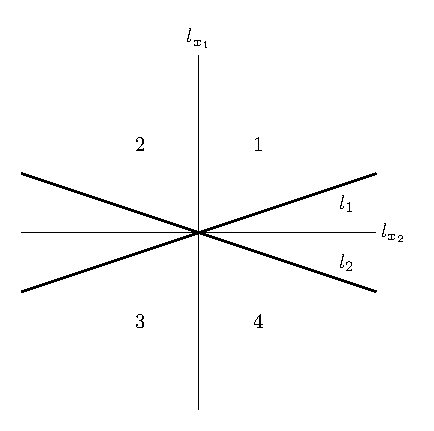
\includegraphics[width=.85\textwidth]{images/4l1234.pdf}
    \end{figure}
    \end{minipage}% <---------------- Note the use of "%"
    \begin{minipage}[t]{.5\textwidth} 
        \vspace{25pt}
        Now we have $n/2$ pairs $(H_1,H_2)$, where $H_i\in S_i$. Let $l_i$ be the intersection of $H_i$ and $x_1x_2$ plane.
        Let $H_{x_i}$ be the linear combination of $H_1$ and $H_2$ s.t. $x_i$ is eliminated.
    \end{minipage}

    { 
    % Now we have $n/2$ pairs $(H_1,H_2)$, where $H_i\in S_i$. Let $l_i$ be the intersection of $H_i$ and $x_1x_2$ plane.
    % Let $H_{x_i}$ be the linear combination of $H_1$ and $H_2$ s.t. $x_i$ is eliminated.
    By the previous lemma, calling oracle on $l_{x_1}$ and $l_{x_2}$ locate $x^*$ with respect to at least one of $H_1$ and $H_2$.}
    \newpage
    Input: $S_1,S_2$ and the pairs.
    \begin{enumerate}
        \item recursively locate $x^*$ respect to $B(d-1)n/2$ hyperplanes($H_{x_i}$) with $A(d-1)$ oracle calls in $S_1$.
        \item locate with respect to a $B(d-1)$-fraction of corresponding paired hyperplanes in $S_2$.
        \item There are still $(1-{B(d-1)}^2)/2$-fraction of hyperplanes for which we do not know the relative position with $x^*$. Run this algorithm on these hyperplanes.
    \end{enumerate}
    This gives the recurrence
    \[
        T(n,d)\leq 3\cdot 2^{d-1}T(n,d-1)+T((1-2^{1-2^d})n,d)+O(nd)
    \]
    with solution $T(n,d)=O(2^{2^d}n)$.
\end{frame}
\begin{frame}{Zemel's conversion}
    Our linear program has \emph{dimension} $n+d$. \href{https://www.sciencedirect.com/science/article/abs/pii/0020019084900140}{Zemel} showed that this kind of problem can be converted to a linear program of dimension $d$.
    \begin{align*}
        \min &\sum_{i=1}^n f_i\\
        s.t. \quad f_i&\geq \alpha_j(a_i\cdot x -b_i)-\beta_j \quad \forall i\in[n], \forall j\\
    \end{align*}
    \mybox[oliver!20]{
        \scriptsize Here is an intuitive way to understand the conversion. One can think the LP above as a $d$-dimensional search problem with $n+d$ hyperplanes. However, the oracle is quite different. The oracle takes the unknown $x^*$ and a hyperplane $H$ as input, returns the relative position by computing the minimal $f_i$.
    }
\end{frame}

\section{Possible Improvements}

\begin{frame}{Other algorithms for fixed dimension LP}
    \begin{figure}
        \centering
        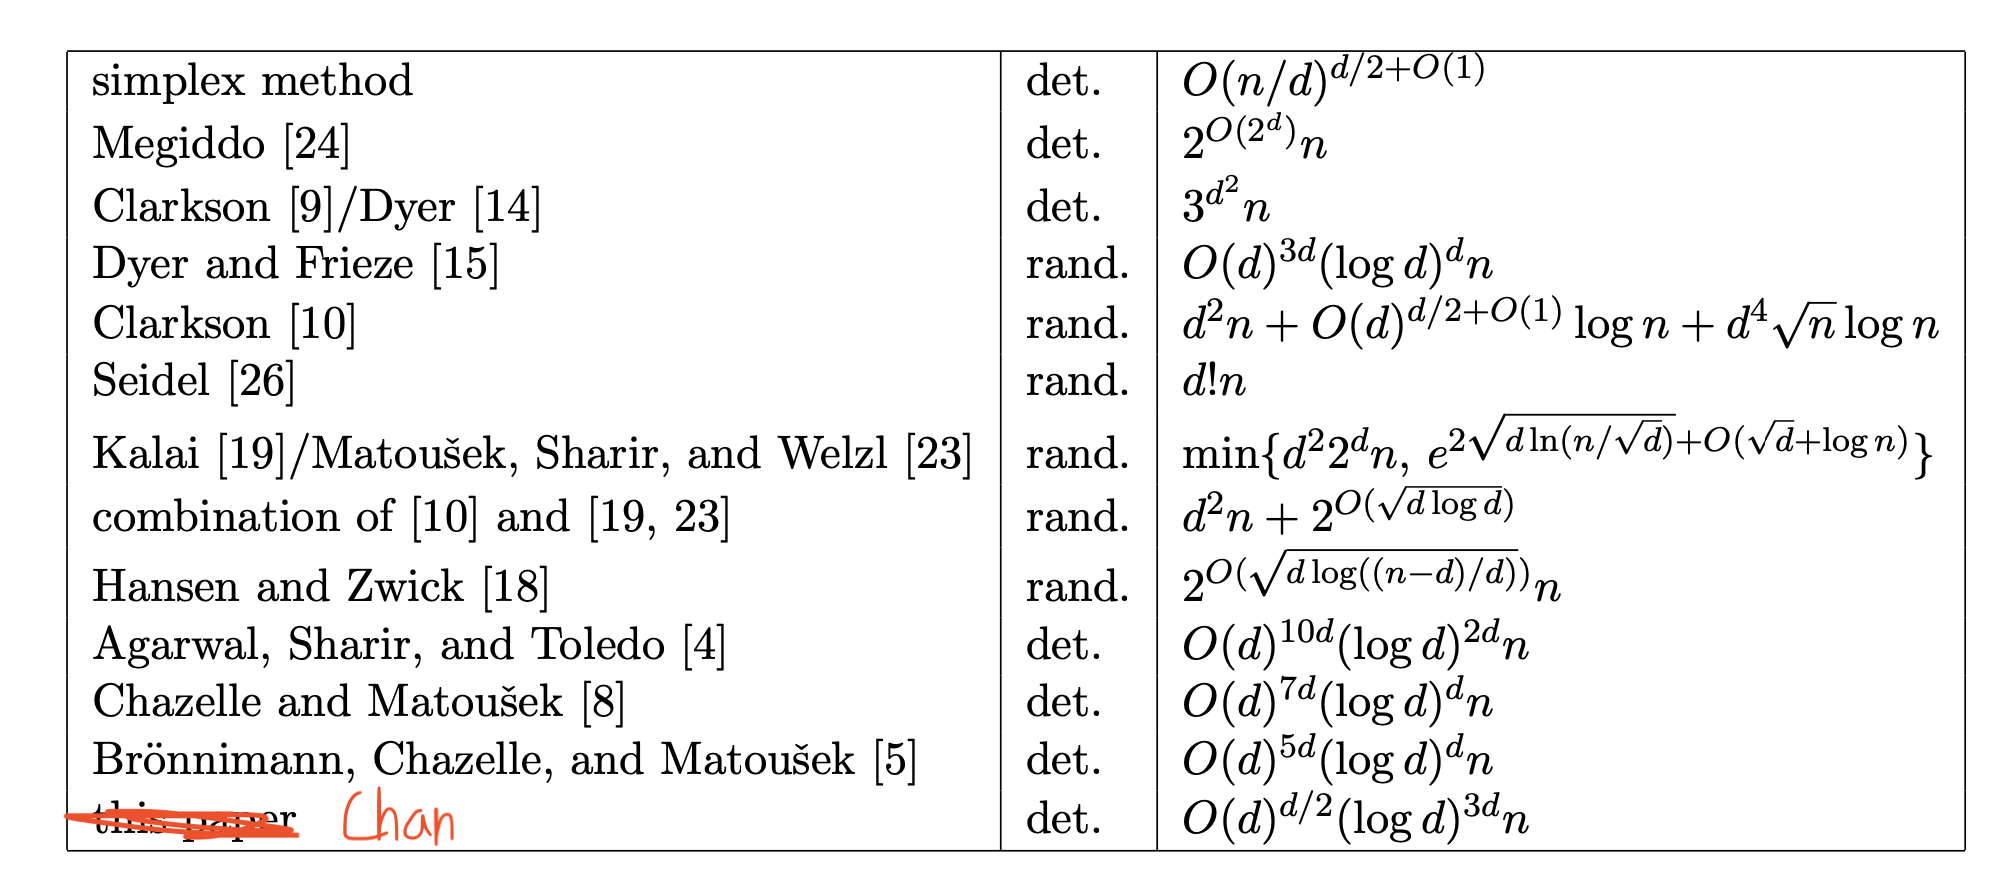
\includegraphics[width=\textwidth]{images/table.png}
        \caption{Algorithms for LP in low dimensions \footnote{table stolen from \url{https://dl.acm.org/doi/10.1145/3155312}}}
    \end{figure}
    \textbf{Can we use faster fixed dimension LP algorithms to get better complexity?}
\end{frame}

\begin{frame}[allowframebreaks]{LP-type problem}
    Algorithms for low dim LP are actually solving a more abstract problem.
    \begin{definition}[LP-type problem]
        Given a set $S$ and a function $f:S\to \R$. $f$ satisfies two properties:%
        \begin{itemize}
            \item Monotonicity: $\forall A\subseteq B\subseteq S, f(A)\leq f(B)\leq f(S)$.
            \item Locality: $\forall A\subseteq B\subseteq S$ and $\forall x\in S$, if $f(A) = f(B) = f(A \cup \{x\})$, then $f(A) = f(B \cup \{x\})$.
        \end{itemize}
    \end{definition}
    Linear programs(minimization) are LP-type problems.

    $B\subseteq S$ is a basis if $\forall B'\subsetneq B, f(B')<f(B)$. A set of `useful' constraints in a linear program is a basis.

    The combinatorial dimension is the size of the largest basis.

    If a LP problem has low dimension, then its combinatorial dimension is low. \textbf{What about the converse?}
    \newpage
    \textbf{Does our LP has low combinatorial dimension?}
    
    No! A basis contains at least $n$ constraints since otherwise some $f_i$ is unbounded.
\end{frame}



\begin{frame}{Aggregate the pwl convex functions}
    % blog posts
\end{frame}

\end{document}